% use lualatex to compile, for some reason xelatex fails for the {Libertinus Serif} font.
\documentclass[11pt]{book}
%\documentclass[11pt]{amsart} % fails on title, date, etc.

% ---------- Fonts (LuaLaTeX / XeLaTeX) ----------
\usepackage{fontspec}
\setmainfont{Libertinus Serif}
%\setmainfont{TeX Gyre Pagella}
%\setsansfont{TeX Gyre Heros}
\setmonofont{Inconsolata}

% ---------- Page layout ----------
\usepackage[a4paper,margin=1.1in]{geometry}

% ---------- Math & theorem setup ----------
\usepackage{amsmath,amssymb,amsthm,mathtools}

\theoremstyle{definition}
\newtheorem{definition}{Definition}
\newtheorem{example}{Example}

\theoremstyle{plain}
%\newtheorem{theorem}[definition]{Theorem}
\newtheorem{theorem}{Theorem}
\newtheorem{lemma}{Lemma}
\newtheorem{proposition}{Proposition}
\newtheorem{corollary}{Corollary}
\newtheorem{exercise}{Exercise}[chapter]



\usepackage{xcolor}
\newtheoremstyle{problemstyle} % name
  {3pt} % Space above
  {3pt} % Space below
  {\normalfont} % Body font
  {} % Indent
  {\bfseries\color{blue}} % Theorem head font
  {.} % Punctuation
  { } % Space after head
  {} % Head spec
\theoremstyle{problemstyle}
\newtheorem{problem}{Problem}


\theoremstyle{remark}
\newtheorem*{remark}{Remark}
\renewcommand\qedsymbol{$\blacksquare$}
% the reflection box
\usepackage[framemethod=tikz]{mdframed}
\theoremstyle{definition}
\newtheorem{reflection}{Reflection}
\mdfdefinestyle{reflectionbox}{
  innertopmargin=\topskip,
  roundcorner=5pt,
  linecolor=cyan,
  backgroundcolor=cyan!20,
}
\surroundwithmdframed[style=reflectionbox]{reflection}
% the reflection box
% quotes
\usepackage[style=english]{csquotes}
\MakeOuterQuote{"}
% quotes

% epigraphs
% I chose epigraph-keys for its simplicity
\usepackage{epigraph-keys}
% epigraphs

%images
\usepackage{graphicx}
\usepackage{float}
\usetikzlibrary{graphs,graphdrawing,arrows.meta,intersections,calc,patterns}
\usegdlibrary{trees,layered}
%images
% ---------- Typography ----------
\usepackage{microtype}

%plots
\usepackage{pgfplots}
%plots

% multiple columns
\usepackage{multicol}
\setlength{\columnseprule}{1pt}
\def\columnseprulecolor{\color{blue}}
% multiple columns
%multirow (tables) using makecell
\usepackage{makecell}
\renewcommand\theadfont{\bfseries}
%multirow (tables) using makecell

%canceling terms
\usepackage{cancel}
%canceling terms

%customize lists
\usepackage{enumitem}
%customize lists

% for dotdiv operator
\usepackage{mathabx}
% for dotdiv operator
% comment out large portions, but document them in source 
\usepackage{comment}
% comment out large portions, but document them in source 

% general-purpose box with counters and labels for referencing
\usepackage{tcolorbox}
\tcbuselibrary{skins}

% Create an environment called "mybox" with an automatic counter
\NewTColorBox[auto counter]{mybox}{o}{
  colback=blue!15!white,
  colframe=blue!75!white,
  fonttitle=\bfseries,
  title=Box \thetcbcounter: #1
}
% general-purpose box with counters and labels for referencing

% the stylized "diagonal" fraction look
\usepackage{xfrac}
% the stylized "diagonal" fraction look

% strikethrough
\usepackage[normalem]{ulem}
% strikethrough

% tbd command
\newcommand{\tbd}{
    \vspace{5mm}
    \textbf{\textcolor{red}{\Large{TBD}}}
    \vspace{5mm}
}
% tbd command
% bib
\usepackage[
  backend=biber,
  style=numeric
]{biblatex}

\addbibresource{refs.bib}
% bib

%macros
%macros
% https://github.com/plk/biber/issues/373
\DeclareBibliographyAlias{movie}{misc}
% https://github.com/plk/biber/issues/373
% ---------- Hyperlinks ----------
\usepackage[hidelinks]{hyperref}

% ---------- Metadata ----------
\title{Notes on \\ \emph{Combinatorial Algorithms, The Art of Computer Programming, Volume 4A Part 1}
\\ \emph{by Donald Knuth \cite{taocp-v4a-p1}}
\\ }
\author{Kedar Mhaswade}
\date{15 Aug 2026}

\begin{document}
\maketitle
\cleardoublepage
\chapter*{}
\thispagestyle{empty} % Remove headers and footers

\vspace*{\fill} % Push the text vertically down the page

\begin{center}
    \textit{I thank Donald Knuth for being the DroNaachaarya for this ekalavya (in spirit but perhaps not ability).}
\end{center}

\vspace*{\fill} % Center the text vertically on the page
\cleardoublepage

\begin{reflection}[Introduction]
    These are the author's highly personal notes based on this book \cite{taocp-v4a-p1}. They may occasionally sound like author's conversation with the reader (or even himself). Even if they are personal and appear in the public domain, they may help the reader, although the author isn't exactly sure how. He wrote them for 0) the love of mathematics and writing 1) \LaTeX{} practice (of writing hopefully readable mathematics, albeit longer than appearing in standard texts), and 2) reliable archival (paper, on which most work is created, tends to get lost) that incurs minimal overhead.

    These notes are interspersed with ``reflection boxes'' like this one. They are meant to express author's `rough' thinking process (mental catharsis of sorts), of which frustration is often an inseparable part. The author writes mostly in first person for an authentic conversational tone.

\end{reflection}

\begin{reflection}[Introduction 2]
    ``Why Knuth now? Don't you have enough going (Carl Smith's book, Boyd-Vandenberghe's book, etc.) already? Don't you realize you are a mere mortal? Knuth's are reference books, not textbooks, don't you know that? Also, you are easily distracted, will you be able to bring your attention to a focus required for meaningful reading of his books?''

    Those were the questions I had to pacify before starting yet another attempt with reading Knuth's books. I was never impressed with Bill Gates's proclamation\footnote{He wanted readers who finish Knuth's books (!) to write to him, presumably for a job!} (and I am less impressed now for reasons similar to Warren Buffett's reasons to end their high-profile friendship), so that's not a motivation.

    So, why now?

    Well, I can readily \emph{blame it on} Dragonfjord's amazing puzzle, \emph{A Puzzle a Day} \cite{apad}. 
    \begin{figure}[H]
      \centering
        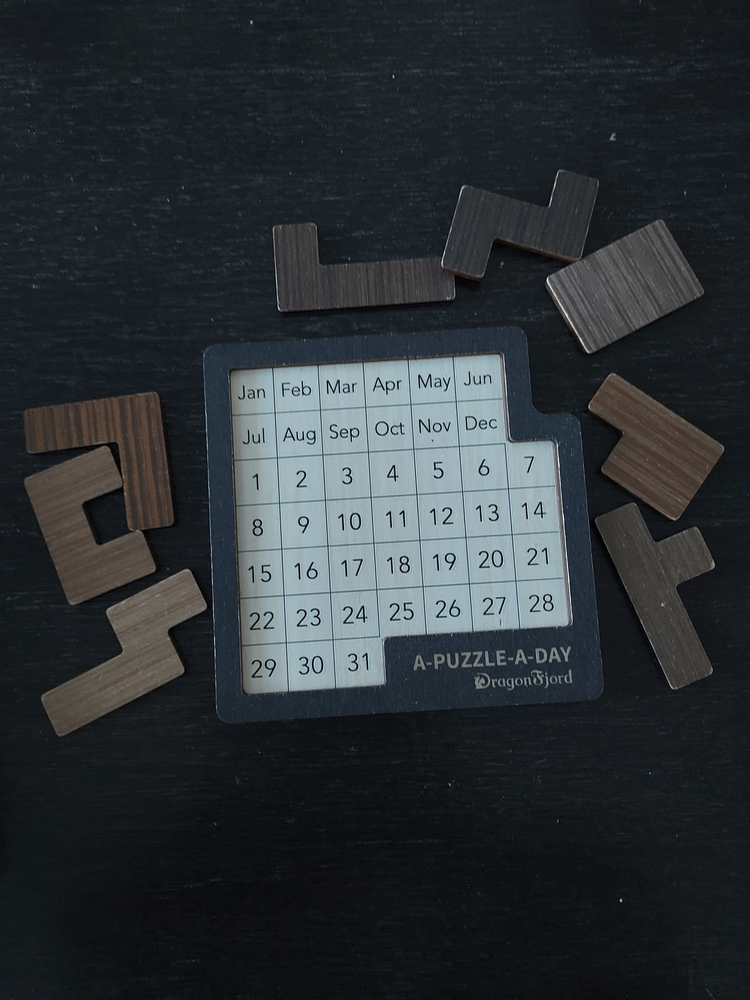
\includegraphics[scale=0.2]{images/apad-pieces-s}
      \caption{The Puzzle Grid and Pieces}
      \label{fig:apad-pieces}
    \end{figure}

    A good friend introduced me to this creative puzzle, and, after spending a few hours on it to `solve various dates' (like in Figure [\ref{fig:apad-15-aug}]), I thought of writing a computer program to solve it.  
    \begin{figure}[H]
      \centering
        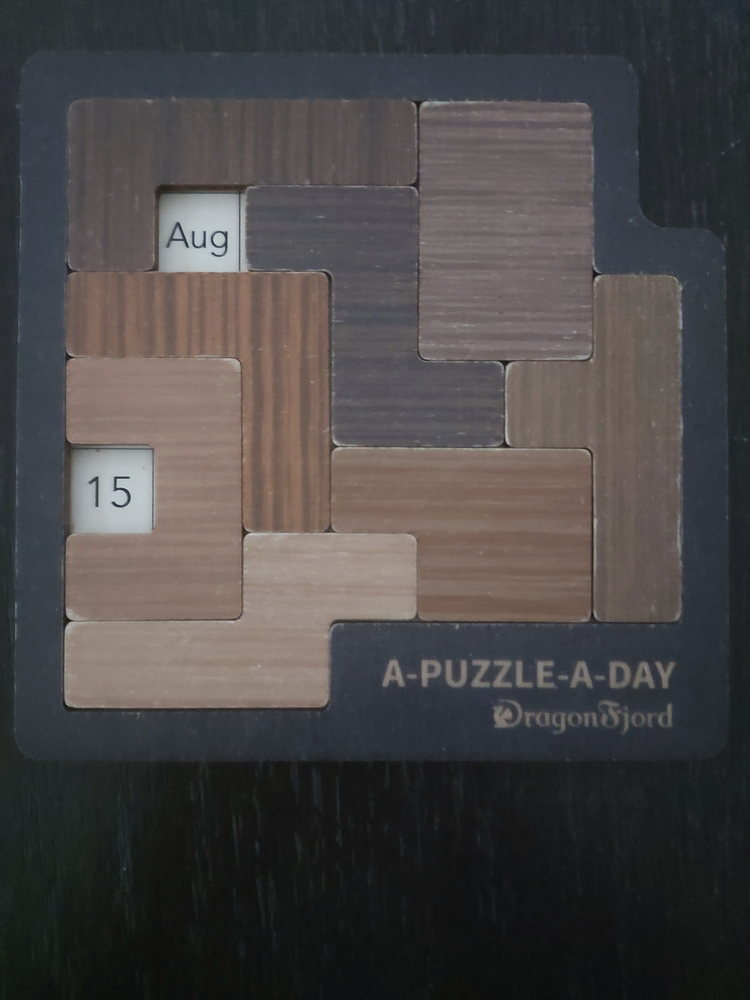
\includegraphics[scale=0.2]{images/apad-15-aug-s}
      \caption{A Solution for 15 August}
      \label{fig:apad-15-aug}
    \end{figure}

    I didn't have to reopen for this computer program the long-longed project of reading algorithms (and solving problems) from Knuth's Volume 4A, which contains the kind of algorithms he likes best. But I did. \textbf{This means delaying writing the program I want to}. So, I decided this: Write the program with what I know of combinatorial algorithms as of today, but also keep reading the book as much (and as consistently) as I can to acquire the combinatorial algorithm techniques. Having a problem to solve also helps analyze the theory from the point of view of an immediate application. 

    The other reason is reading Knuth is almost always an enlightening experience. He takes you on a grand scientific, philosophical, historical, cultural, and, of course, mathematical ride. He cares about every word he puts in his books. And he's been caring about his exposition since 1962, when he was about 24. I know no other writer with such obsession. He wrote the books, wrote software to beautifully typeset them, and he is still writing his books at 88. I feel like it is my duty to at least read parts of what he wrote. I want to do this not for the obligation, but for the love.

    I have an \emph{O'Reilly Learning} subscription that enabled me to access the digital copy \cite{taocp-v4a-p1-digital} of this book. I am reading the digital release of July 2026. Knuth is wary of reproductions of his books because they introduce errors; but this one appears faithful. I hope it has addressed all the errata so far!
\end{reflection}

\section{Preface}

\epigraph[author={Paul Halmos}, source={I Want to be a Mathematician \cite{halmos-iwtbam}}, width={0.7\textwidth}]
{
    Audience, level, and treatment--a description of such matters is what prefaces are supposed to be about.
}
\begin{reflection}
    Knuth provides a thorough overview of what's to come. This is indeed a very well-written preface! What's more, his narrative resembles a story. He explains why it is important to write good combinatorial algorithms (which he loosely, but incisively, defines) despite astounding progress in processor speeds and abundance of computer memory. Simply put, computers have consistently become faster, but (combinatorial) problems have become much bigger in comparison. Learning these algorithms is in part about appreciating the scale of such problems.
\end{reflection}
\begin{definition}[Loosely Speaking \dots]
    \label{def:combinatorial-algorithms}
    Combinatorial algorithms can be defined informally as techniques for the high-speed manipulation of combinatorial objects such as \emph{permutations} or \emph{graphs}. We typically try to find \emph{patterns} or \emph{arrangements} that are the best possible ways to satisfy certain constraints. The number of such problems is vast, and the art of writing such programs is especially important and appealing because a single good idea can save years or even centuries of computer time.
\end{definition}

\begin{lemma}[Floyd's Lemma]
    Problems that seemed to need $O(n^3)$ operations could actually be solved in $O(n^2)$; problems that seemed to require $O(n^2)$ could be handled in $O(n\log n)$; and $n\log n$ was often reducible to $O(n)$.
\end{lemma}

\epigraph[author={Don Knuth},source={Preface to Taocp Volume 4A}]{
    Many combinatorial questions that I once thought would never be answered during my lifetime have now been resolved, and those breakthroughs have been due mainly to improvements in algorithms rather than to improvements in processor speeds.
}

\begin{reflection}
    So, the emphasis is on ``finding \emph{patterns} or \emph{arrangements} that are the best possible ways to satisfy constraints.''

    This principle sounds applicable regardless of the size of a combinatorial problem, or any problem, where constraints are inherent in the problem definition. In any computer program, we must model what is given in terms of structures (data structures) and operations (algorithms) on them. In many problems, choices are obvious. In combinatorial problems, perhaps we have multiple choices to represent what is given, and the art is in choosing the representation, pattern, or arrangement (and realize it in terms of data structures and algorithms) with the biggest payoff.

    In some sense, this is the same requirement from an `optimal algorithm' to solve any computational problem, not just combinatorial. However, in combinatorial problems, identifying optimal patterns seems to be trickier than in other cases. 
\end{reflection}


\epigraph[author={Don Knuth},source={Preface to Taocp Volume 4A}]{
    The great combinatorial fermentation of 1975 has continued to churn, as more and more people have begun to participate. New ideas improve upon the older ones, but rarely replace them or make them obsolete. So of course I've had to abandon any hopes that I once had of being able to surround the field, to write a definitive book that sets everything in order and provides one-stop shopping for everyone who has combinatorial problems to solve. The array of applicable techniques has mushroomed to the point where I can almost never discuss a subtopic and say, ``Here's the final solution: end of story.'' Instead, \emph{I must restrict myself to explaining the most important principles that seem to underlie all of the efficient combinatorial methods that I've encountered so far}. At present I've accumulated more than twice as much raw material for Volume 4 as for all of Volumes 1-3 combined.
}

\begin{reflection}
    Knuth has said somewhere that he's like a cataloger. That position is evident. He wants to `freeze the pace of development' and finish his books once and for all. Of course, he knows that that is not possible. Many researchers keep pushing the limits of efficiency of algorithms. Even in the age of A.I., that seems to hold. Our ways might need a appropriate tool upgrade (e.g., use of Claude Code, which Knuth has demonstrated in \cite{claude-cycles}). Nietzsche's words--He who has a why can deal with almost any how--reverberate in my ears. Knuth has amazing clarity or purpose. Questions like ``Should I adopt Claude Code?'' or ``Should I employ A.I. to prove theorems?'' do not create any crisis for him. He uses Claude as a tool. He solved a hard problem using Claude and went back to solving other problems. A.I. does not bother him, although he does seem to acknowledge its power. 

    Since understanding the A.I. revolution as a researcher is my goal in the medium term, I will write about it briefly.

    In recent months, the question ``How to think about A.I.?'' has troubled me. A lot. There are a lot of noise, uncertainty, and lies. However, I tend to be on the side of progress, not of A.I. Luddites. The A.I. policy issue is a big one, it poses many ethical and existential concerns. However, I don't want to oppose it. I want to learn it. I want to understand what makes it work. It's a monster, and so I need to choose a tiny area as far as research is concerned. 

    As a policy, there's no point in resisting the impending change. We must adapt. If we are going to perish as a species no matter what, I might as well learn A.I. and perish.

    We value opinions of those whose work and values matter to us. Knuth is one such person. He says the following in his paper:

    \epigraph[author={Don Knuth},source={Claude Cycles \cite{claude-cycles}}]{
        Shock! Shock! I learned yesterday that an open problem I’d been working on for several weeks had just been solved by Claude Opus 4.6--Anthropic’s hybrid reasoning model that had been released three weeks earlier! It seems that I'll have to revise my opinions about `generative AI' one of these days.
    }

    Many (countless?) researchers in science and mathematics are now heard echoing this sentiment. A.I. is cracking hard `Erd\H{o}s Problems.' There is tremendous business interest in A.I. Conscientious top A.I. researchers (although while working for wealthy companies) are touting its powers, A.I. is being used increasingly by Nobel laureates and Fields medalists. So, I don't have to give special importance to Knuth's opinions. But I do. Whereas I want to listen to his opinions about generative A.I. in detail, it is clear that he's in awe of its capacity: Better (A.I.) models are going to be irreplaceable as our alleys\footnote{I hope they don't `take over'!}. I just don't know how these models will stop being used and enhanced. Some apocalypse may wipe them out, but then a significant portion of us all may get wiped out. This is where it goes into A.I. policy and there's a lot to speculate there. 

    I don't want to speculate. Knuth's example is motivating because he wants to embrace A.I. to do what he has always wanted to do: Write readable computer programs to solve hard problems. He is the professor emeritus of `The Art of Computer Programming' at Stanford. The position apparently matters. However, his dedication matters more. Therefore, he can revise his opinions about A.I. without being intimidated or threatened by its onslaught.

    Is his example a good one to `emulate'? No. He is a genius. And we don't want to emulate any one person. We learn from others what makes sense to us and constantly make ourselves our better versions. What I take from Knuth is the so-called `renaissance attitude'--an attitude of learning to solve interesting natural or artificial problems of humongous scale with apparently nonchalant disregard for convention. Of course, I want to remain grounded and modest. It's important not to get carried away by Knuth's example.

    Is my `A Puzzle a Day' (See \cite{apad}) a problem of such gigantic scale? Perhaps not in this concrete form. However, it can be made arbitrarily complex. It is a specific case of the `tiling problem' which concerns tiles--also called Polyominoes (See \cite{polyominoes})--and their packing in a grid. The puzzle (See Figure [\ref{fig:apad-pieces}]) has seven (of the 12 free) pentominoes (See \cite{free-pentominoes}) and one hexomino (of the 35 free possible) (See \cite{free-hexominoes}). I hypothesized that before making the wooden puzzle, the creators had to ensure that every date is solvable\footnote{For example, 15 Aug is solvable when the 8 polyominoes cover every square other than `15' and `Aug' as shown in Figure [\ref{fig:apad-15-aug}].}. I wonder how one can ensure that without writing a computer program. Can the puzzle be solved with only pentominoes? Can the puzzle be solved with only pentominoes?

    So, whereas I am searching the one research area to which I can dedicate all my time and energy unhesitatingly, something tells me that this is the right thing to do in the short term: 1) Study combinatorial algorithms. 2) Don't hesitate to use A.I. tools; don't be a Luddite. That inner voice may just be intuition or even confused debris accumulated in my subconscious, but there's a poorly specified conscious effort to reach this stage. My intuition was perhaps never as strong as the great Ramanujan's.

    One issue concerns the choice of A.I. models. Some say that we must use the cutting-edge models, which are charged at a premium. The free-tier models are much less capable than premium models. This may be a marketing gimmick. However, all the recent cases where A.I. models showed creative problem-solving skills or solved hard problems almost single-handedly, have used the cutting-edge commercial or open-source models. There's no point in staying on free-tier models if your problems require models with `advanced reasoning capabilities.' 

    Okay then! I am all set.
\end{reflection}

\epigraph[source={About What's Left Out}]{
    [I leave out Computational geometry, polyhedral combinatorics, linear programming, algorithms almost exclusively for the `asymptotic case' \dots] Purely combinatorial developments are easier for me to understand \dots\;In The Art of Computer Programming I tend to give short shrift to any methods that I would never consider using myself in an actual program.
}

\epigraph[source={Structure of the presentation}]{
    [Problems or Techniques? \dots] The main decision that I needed to make when planning how to present this material was whether to organize it \textbf{by problems or by techniques}. \dots I finally decided that a mixed strategy would work better than any pure approach.
}

\epigraph[source={About Stanford GraphBase}]{
    Another downloadable resource, a collection of programs and data called The Stanford GraphBase, is cited extensively in the examples of this book. Readers are encouraged to play with it, in order to learn about combinatorial algorithms in what I think will be the most efficient and most enjoyable way.
}
\begin{reflection}
    Graphs are versatile. People have dedicated their lives studying, applying, and implementing graphs. Perhaps studying the Stanford GraphBase will help me realize this one-time fascination of me. Let's see.

    Knuth also refers to his computer programs and urges readers to study them. See \cite{knuth-programs}.

    He also uses a consistent notation that he documents. See the file \texttt{appendix-b-notation.pdf} in this folder.
\end{reflection}


\epigraph[source={Notes on the Exercises}]{
    The exercises in this set of books have been designed for self-study as well as for classroom study. It is difficult, if not impossible, for anyone to learn a subject purely by reading about it, without applying the information to specific problems and thereby being encouraged to think about what has been read. Furthermore, we all learn best the things that we have discovered for ourselves. Therefore the exercises form a major part of this work; a definite attempt has been made to keep them as informative as possible and to select problems that are enjoyable as well as instructive.
}
\epigraph[source={Notes on the Exercises--2}]{
    Some exercises are preceded by an arrowhead, $\blacktriangleright$; this designates problems that are especially instructive and especially recommended. Of course, no reader/student is expected to work all of the exercises, so those that seem to be the most valuable have been singled out. (This distinction is not meant to detract from the other exercises!) Each reader should at least make an attempt to solve all of the problems whose rating is 10 or less; and the arrows may help to indicate which of the problems with a higher rating should be given priority.

Several sections have more than 100 exercises. How can you find your way among so many? In general the sequence of exercises tends to follow the sequence of ideas in the main text. Adjacent exercises build on each other, as in the pioneering problem books of P\'olya and Szeg\H{o}. The final exercises of a section often involve the section as a whole, or introduce supplementary topics.
}

Summary of Exercise Ratings:
\begin{enumerate}
    \item $\blacktriangleright$: Recommended
    \item M: Mathematically oriented.
    \item HM: Requiring `higher math'
    \item 00: Immediate
    \item 10: Simple (one minute)
    \item 20: Medium (quarter hour)
    \item 30: Moderately hard
    \item 40: Term project
    \item 50: Research problem
\end{enumerate}

\begin{reflection}[It's humbling]
    Reading Knuth is exciting, but it is also intimidating. However, I feel humbled looking at all the natural and artificial problems that he discusses. There are only a handful people who have read many (any?) of his books and learned (and implemented) the algorithms and solved problems from them. That's understandable. It's a big commitment. As long as there's joy, the endeavor is worth the effort. Some have also treated his books as reference books to be consulted only when confronted with a problem they are solving. That place, however, has now been taken by the Internet, the search engines, and Wikipedia (and now perhaps A.I. models). 

    Now, you experience his books only for the joy of the struggle.
\end{reflection}


\chapter*{Combinatorial Searching}

\epigraph[author={Robert Tarjan}]{
    The field of combinatorial algorithms is too vast to cover in a single paper or even in a single book.
}
\epigraph[author={Sam Loyd Jr.}]{
    While jostling against all manner of people it has been impressed upon my mind that the successful ones are those who have a natural faculty for solving puzzles. Life is full of puzzles, and we are called upon to solve such as fate throws our way.
}

\begin{reflection}
    The Sam Loyd Jr. quote above is apt. While facing one's life, one can enjoy the natural and artificial problems and puzzles that come our way, many a time, by chance. `Success' is often relative, but the joy may be absolutely real.

    Of those puzzles, combinatorial puzzles such as \emph{A Puzzle a Day} (Figure [\ref{fig:apad-pieces}]) are particularly interesting. The creativity of the puzzle creator is appealing. `Computation' exudes from combinatorial puzzles. When the amount of computation to perform slightly overwhelms the human mind, the puzzle becomes a lasting joy to solve. With practice, one can get better at discerning certain patterns more quickly. Doing something progressively more quickly gives more joy to some.

    However, I have always felt that solving combinatorial puzzles is somewhat mechanical. When solving such puzzles demands an exhaustive search, nothing is more attractive than a correct algorithm and its readable (literate?) implementation. I got that joy when I wrote a computer program to solve combinatorial problems in arithmetic such as this: How can you make 24 using the numbers 1, 3, 4, and 6 exactly once each and the four basic arithmetic operations ($+,-,\times,\div$) any number of times? (See \cite{24-problem}).
\end{reflection}

\begin{definition}[Combinatorics]
    Combinatorics is the study of the ways in which discrete objects can be arranged into various kinds of patterns. 

\end{definition}
\begin{example}
    For example, the objects might be $2n$ numbers $\{1,1,2,2,\dots,n,n\}$, and we might want to place them in a row so that exactly $k$ numbers occur between the two appearances of each digit $k$. When $n=3$ there is essentially only one way to arrange such `Langford pairs,' namely $231213$ (and its left-right reversal); similarly, there's also a unique solution when $n=4$. 
\end{example}










\printbibliography

\end{document}
